\documentclass{article}

\usepackage[numbers,sort &compress]{natbib}
\usepackage[english]{babel}
\usepackage[utf8]{inputenc}
\usepackage{amsmath,amssymb}
\usepackage{parskip}
\usepackage{graphicx}
\usepackage[utf8]{inputenc}
\usepackage[english]{babel}
 
\usepackage[nottoc]{tocbibind}

% Margins
\usepackage[top=2.5cm, left=3cm, right=3cm, bottom=4.0cm]{geometry}
% Colour table cells
\usepackage[table]{xcolor}

% Get larger line spacing in table
\newcommand{\tablespace}{\\[1.25mm]}
\newcommand\Tstrut{\rule{0pt}{2.6ex}}         % = `top' strut
\newcommand\tstrut{\rule{0pt}{2.0ex}}         % = `top' strut
\newcommand\Bstrut{\rule[-0.9ex]{0pt}{0pt}}   % = `bottom' strut

%%%%%%%%%%%%%%%%%
%     Title     %
%%%%%%%%%%%%%%%%%
\title{Reinforcement Learning with Initialized Policy }
\author{Zihan Ding}
\date{\today}

\begin{document}
\maketitle

\tableofcontents
%%%%%%%%%%%%%%%%%
%   Problem 1   %
%%%%%%%%%%%%%%%%%

\begin{abstract}
How can we apply reinforcement learning algorithms for robot control in most efficient way?
\end{abstract}
\section{Background}\label{Background}


\section{Reinforcement Learning Algorithms}
\subsection{Discrete and Continuous Action Space}
\subsection{Deterministic and Non-deterministic Policy}
\subsection{Present Algorithms}
\subsubsection{REINFORCE}
\subsubsection{Actor-Critic}
\subsubsection{Q-learning}
\subsubsection{DQN}
\subsubsection{DDPG}
\subsubsection{TRPO}
\subsubsection{PPO}






\section{Efficient Reinforcement Learning across tasks}
\subsection{Environment}
In this work, we apply reinforcement learning algorithms on the \textit{Reacher} task. As shown in Fig.1, the goal of \textit{Reacher} task is to let the end of `reacher'  agent to be as close as possible to the positions with highest rewards.
\begin{figure}[htbp]
	\centering
	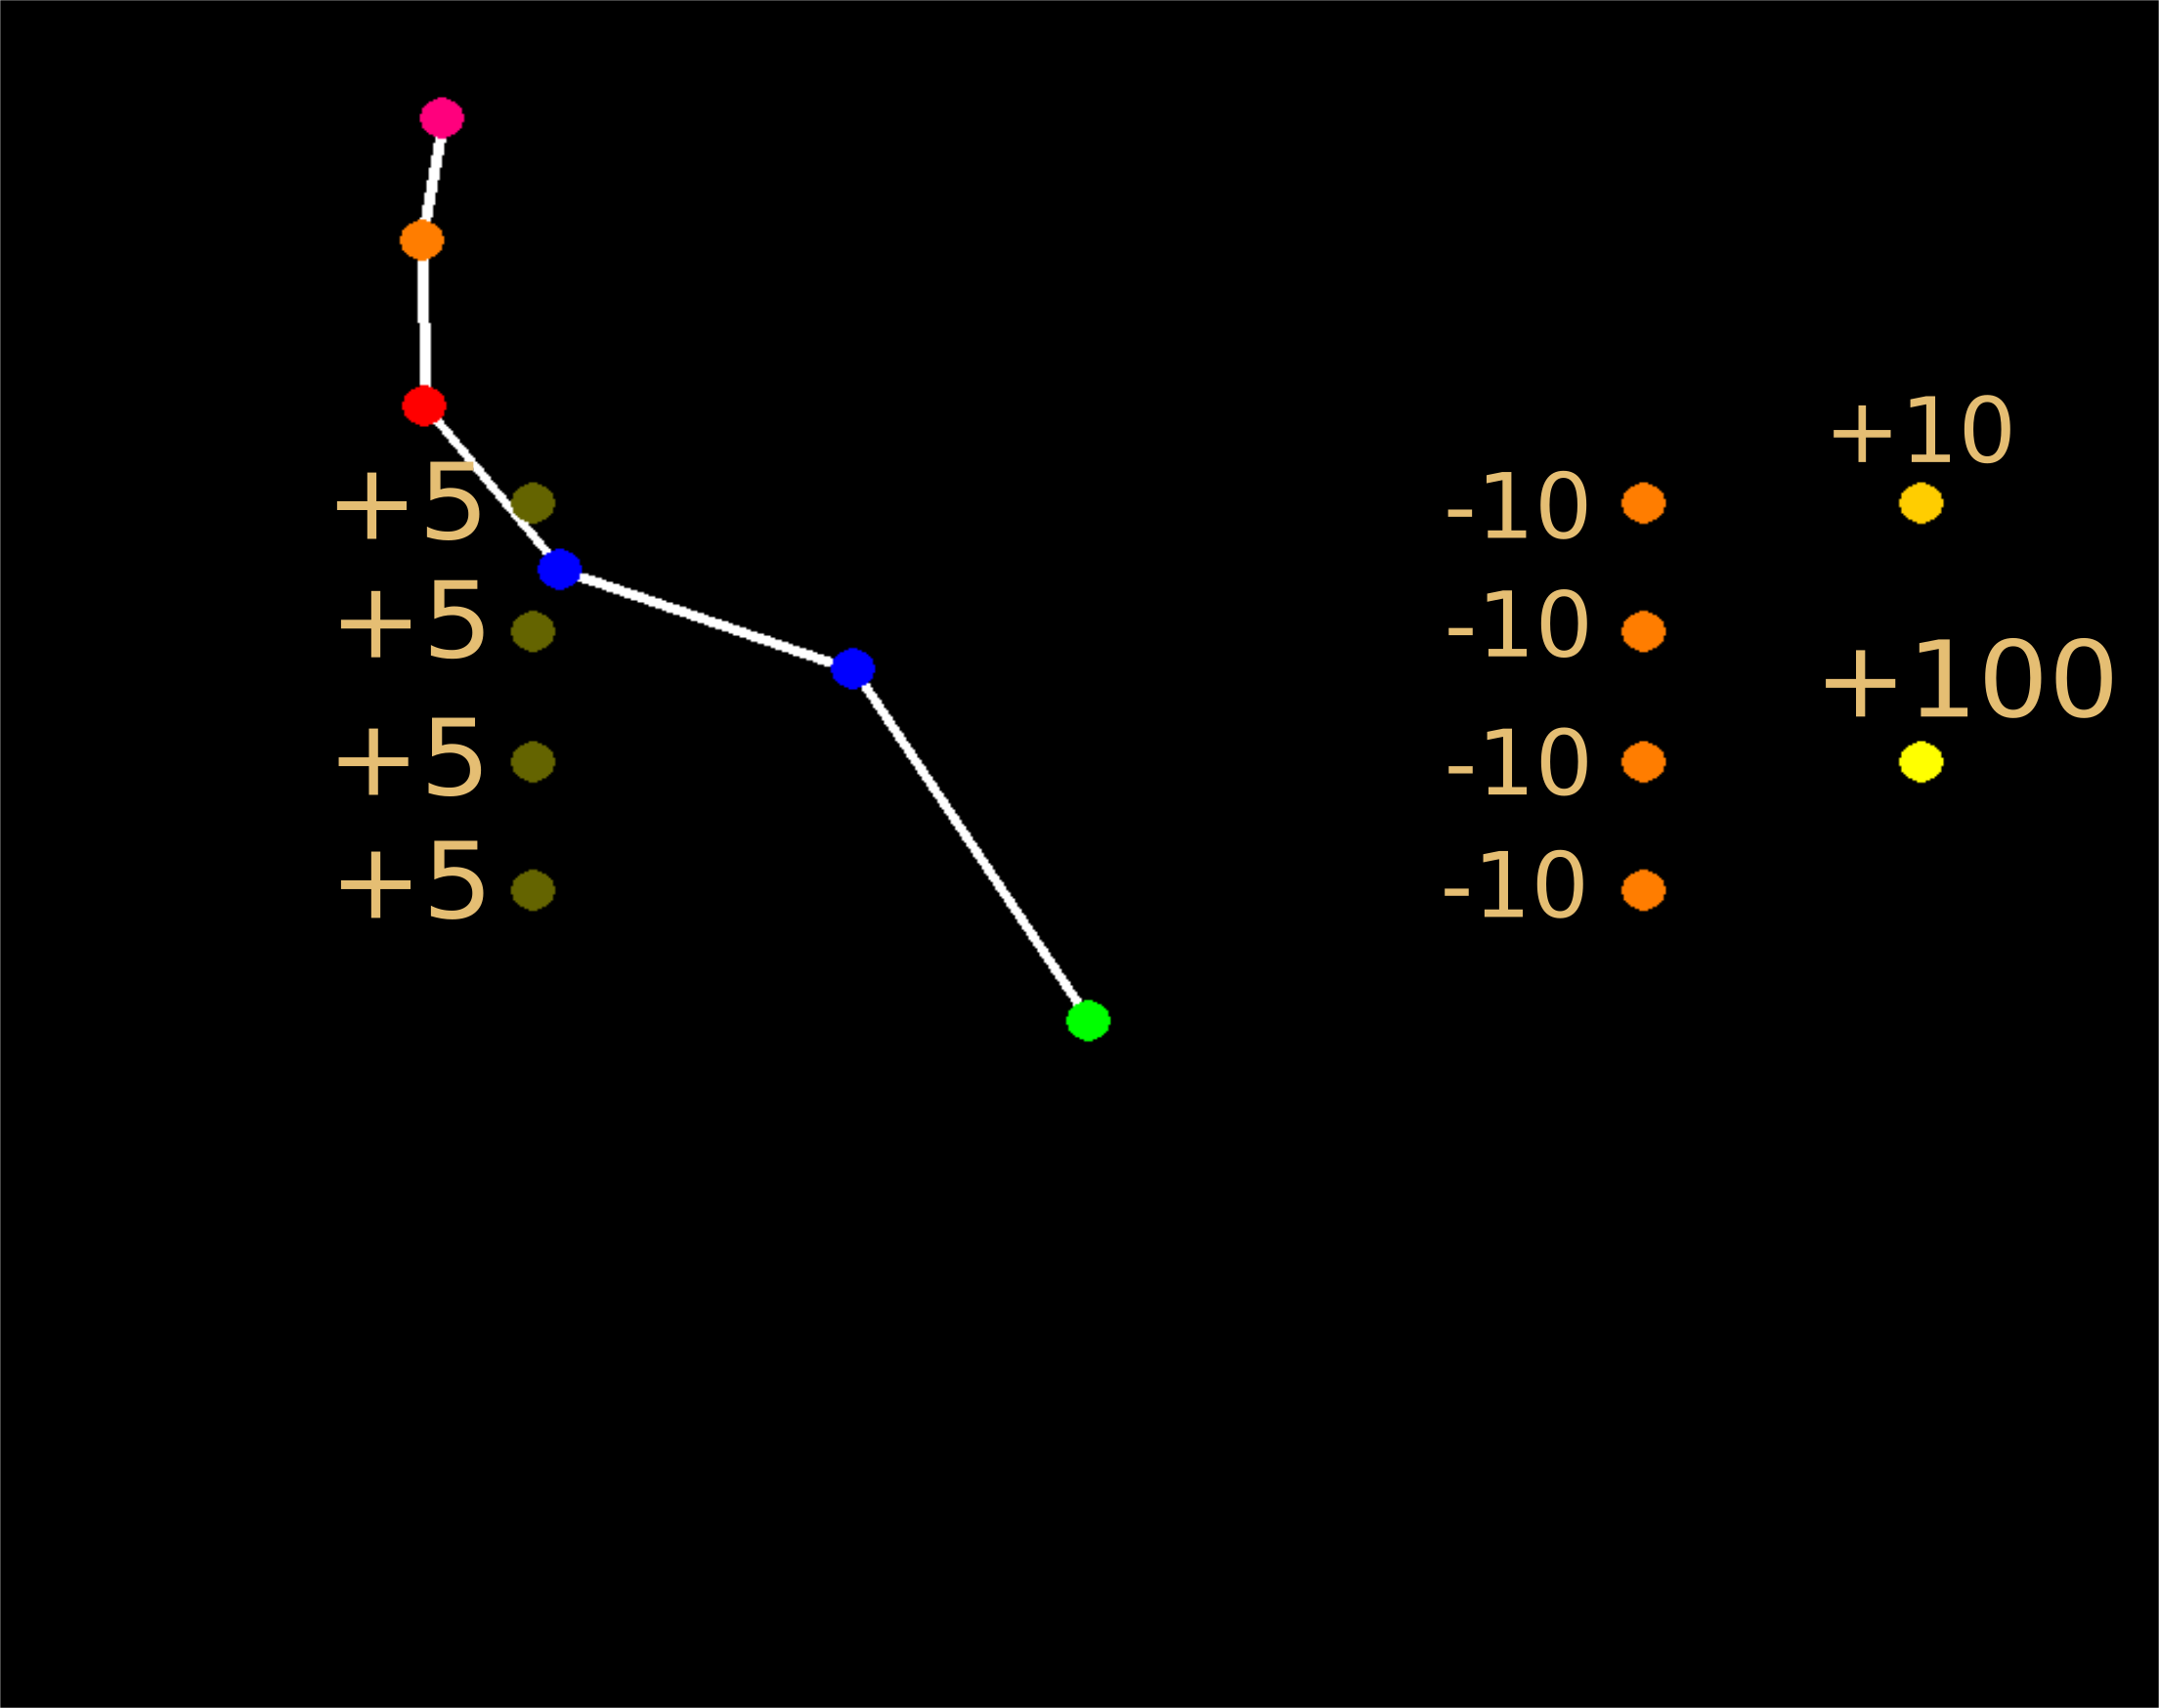
\includegraphics[scale=0.2]{img/reacher.png}
	\caption{\textit{Reacher} task with 5 joints and several reward/penalty positions}
	\label{fig:universe}
\end{figure}

\subsection{Initialized Reinforcement Learning with Supervised Learning Policy}
Reinforcement learning algorithms usually take a long time to achieve a good policy for a specific task. And the policy always needs to be re-trained if the settings of the task are changing, even if slightly. 

There are several ways to improve the learning efficiency of reinforcement learning algorithms. One promising way is to initialize the reinforcement learning policy with a pre-trained policy. And this is especially effective when the pre-trained policy is trained on a similar task with the one the reinforcement learning is trying to solve. Moreover, if the pre-trained policy is trained across the task space containing all possible settings of a specific task that the RL is solving, it can leverage the learning performance of RL for all tasks defined in this task space.
\subsubsection{Task Specification}
In our model, we try to initialize RL with sub-optimal policy pre-trained before the RL process, and the policy is trained with supervised learning with expert trajectories sampled from inverse kinematics on \textit{Reacher} tasks. 

The task space in our model is defined to be the same `reacher' structure with one target point at different positions. The number of joints of `reacher' is chosen to be 3 with length between each pair of joints to be 200, 140 and 100, respectively. The screen size is 1000 and the fixed start point of the `reacher' is at the center of the map. The target position is sampled from a random distribution within the allowed area.
\begin{figure}[htbp]
	\centering
	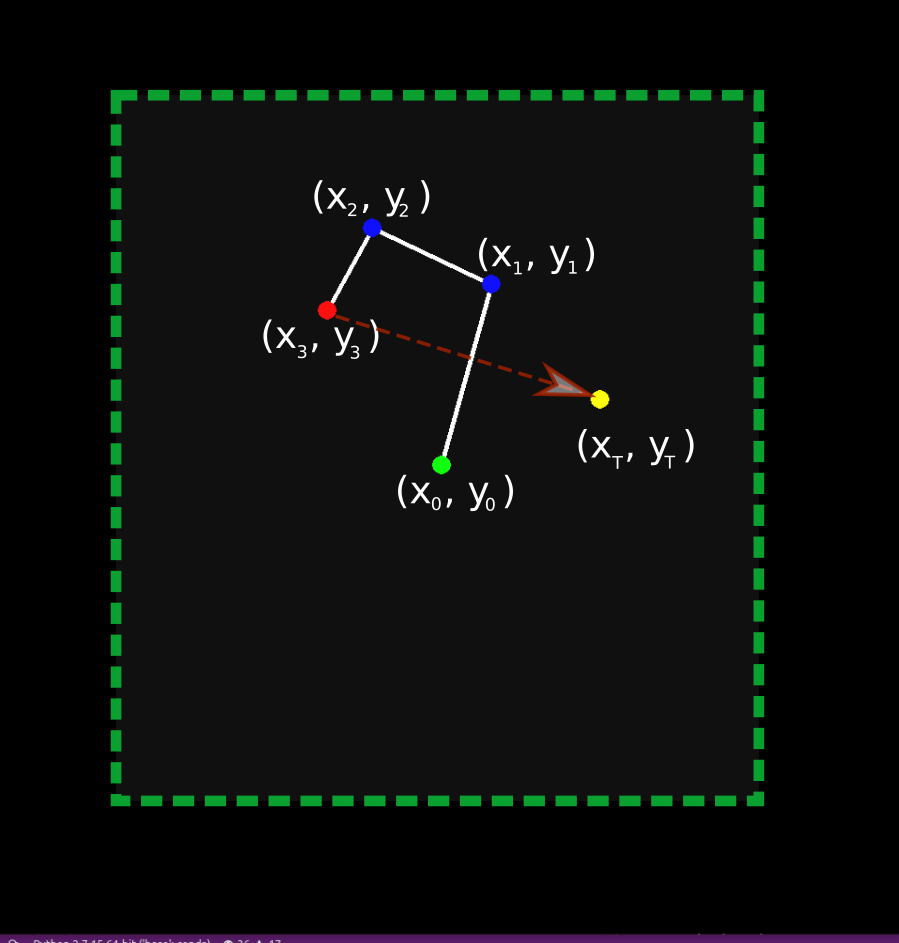
\includegraphics[scale=0.3]{img/reacher1.png}
	\caption{\textit{Reacher} task with three joints and one target point of different possible positions. The green dashed line is the area of potential target positions in the task space.}
	\label{fig:universe}
\end{figure}
The reward function for each step is defined as:
\begin{equation}
 R=\frac{R_0}{\sqrt{(x_3-x_T)^2+(y_3-y_T)^2}+1}, 
\end{equation}
where $R_0=100$ is the maximum of reward value, so $R\in(0,100]$

\subsubsection{Inverse Kinematics}

\subsubsection{Supervised Learning for Initialization Policy}
We apply a neural network of 5 layers to train an initialization policy, with the data generated from inverse kinematics. The inputs of neural network are positions of joints and position of the target.  Each hidden layer contains 100 nodes and uses ReLu as activation function. The output layer is Tanh activated with a scaling factor of 360, to make outputs range from -360 to 360 degree as a reasonable action value of the joints. The AdamOptimizer is applied with stochastic gradient descent in the training process. The training curve is shown in Fig. 3. Note that the y-axis is transformed to be in range [-1,1] instead of [-360, 360] as the mean squared error per action value .
\begin{figure}[htbp]
	\centering
	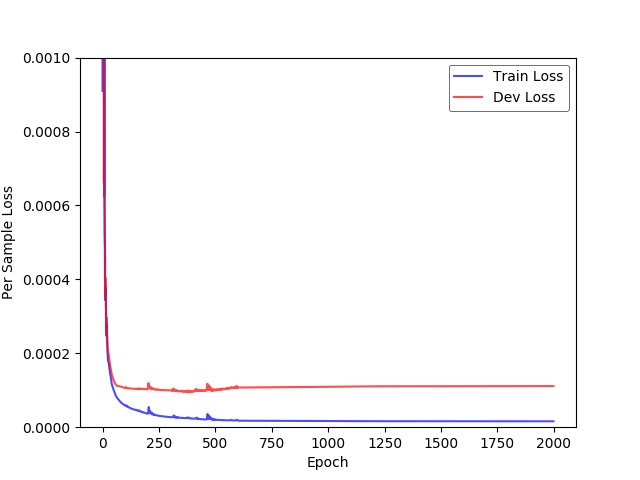
\includegraphics[scale=0.8]{img/supervised.png}
	\caption{Training curve of supervised learning with data from inverse kinematics.}
	\label{fig:universe}
\end{figure}

\subsubsection{DDPG with Initialization Policy -- General Process}
We apply the DDPG algorithm for the task, and show the comparisons with or without initialization for the policy.

The DDPG algorithm contains four neural networks: the actor network, the critic network, the target-actor network, and the target-critic network. For initializing the DDPG, we define the actor network and target-actor network to have exactly the same structure as the network in supervised learning. 

Initialization process of DDPG with supervised learning policy are as follows: 
(1). the weights of pre-trained supervised learning policy are loaded into the actor network and the target-actor are updated immediately; (2). samples are generated with initialized but frozen actor network with noise to pre-train the critic network; (3). train both the actor and critic network (also the target-actor and target-critic networks). Experiments show that the second step is non-trivial process for effective training DDPG with initialization. Details are explained in Sec. \ref{pretrain}.

Comparison of initial learning performances of DDPG with and without initialization policy on \textit{Reacher} task are shown in Fig. 4. The DDPG with initialization policy could significantly outperforms the one without initialization. 

\begin{figure}[htbp]
	\centering
	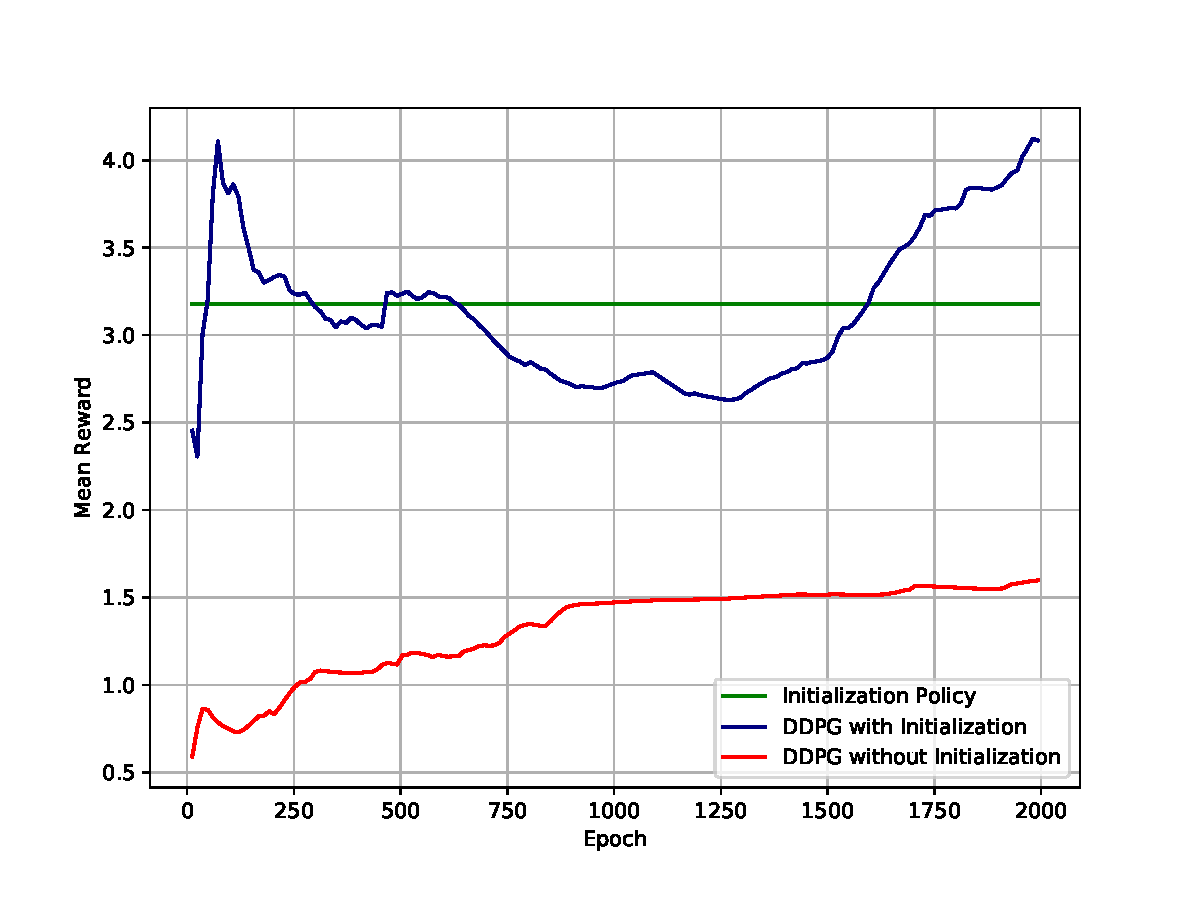
\includegraphics[scale=0.8]{img/ddpg_compare1.pdf}
	\caption{Comparison of initial learning performances of DDPG with/without initialization policy on \textit{Reacher} task. The green line is the mean reward of initial policy trained with supervised learning. The blue line and red line are mean rewards of DDPG with and without initialization in initial 2000 training epochs . }
	\label{fig:universe}
\end{figure}

There are several key components in initializing the RL with supervised learning policy affecting the performance of initialized RL (DDPG), including the scale of action noise in initialized RL, different ways of normalization in supervised learning and RL, learning rates of the actor and the critic in initialized RL, number of steps of single episode and so on. Improper settings of all above factors will affect the initialization policy to be effective for RL process. Some general intuitions about making the initialization more effective for RL are like: ensuring the inputs and outputs of the replaced policy from initialization to be as similar as possible between the supervised learning and RL, therefore applying the same input and output normalization to make sure they are of the same ranges of value, the same initial positions for each episode in `Reacher' and the same maximum length of single episode in supervised learning and RL, etc. 

\subsubsection{DDPG with Initialization Policy -- Choice of Noise}
Noise is an important factor for RL learning process. For initialized policy $\pi_i$ trained with expert trajectories, the optimal trajectory for the same task should be some neighboring trajectories of the initialized trajectory, which means the difference of optimal policy $\pi^*$ and $\pi_i$ should be within a small range $\epsilon$,
\begin{equation}
	D_{KL}(\pi^*||\pi_i)<\epsilon
\end{equation}
This can be derived easily by $(\pi^*(a^*|s_t)- \pi_i(a^*|s_t))<\delta$, where $a^*$ is the optimal action for state $s_t$. However, if we consider another initial policy $\pi'_i$ which is not as good as $\pi_i$, then $(\pi'^*(a^*|s_t)- \pi_i(a^*|s_t))<\delta'$ and $\delta'>\delta$, also we have $D_{KL}(\pi^*||\pi'_i)<\epsilon'$ and $\epsilon'>\epsilon$. In order to handle different initialization policies like $\pi$ or $\pi'$, we need to apply different noise for a better learning performance.

Generally, a larger noise scale or larger probability to have a noise action will help worse policy $\pi'$ to have larger chances to sample an optimal action. We can testify the case of larger probability of have a noise through $\epsilon$-greedy policy, as shown in Fig. \ref{fig:noise}. The $\epsilon$-greedy policy is defined as follows:
\begin{equation}
\pi(a|s)=\left\{
\begin{aligned}
&1-\epsilon+\frac{\epsilon}{|A(s)|}, &a=a* \\
&\frac{\epsilon}{|A(s)|}, &a\neq a*
\end{aligned}
\right.
\end{equation}
In Fig. \ref{fig:noise}, the $\epsilon$-greedy policy can be regarded as a uniform distributed noise on the possible range of action value. It shows that the noise helps the initial policy to have a larger probability to sample the optimal action $a^*$, when the initial policy has a relatively large difference from the optimal policy, which is the case of $\pi'$ with the KL-divergence upper bound  $\epsilon'>\epsilon$.
\begin{figure}[htbp]
	\centering
	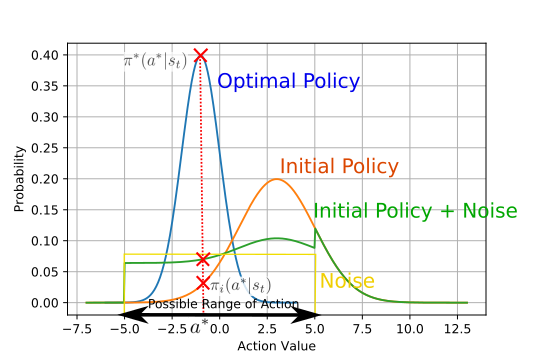
\includegraphics[scale=0.8]{img/noise2.png}
	\caption{A figure showing why adding noise would help for exploring better actions, with noise type of $\epsilon$-greedy policy. Suppose the initial policy and the optimal policy are Gaussian distributions with different means and variances, and the noise is a uniform distribution within specific range (range of possible action value). The figure shows how the noise of $\epsilon$-greedy helps to increase the possibility for non-optimal policy to sample the optimal action }
	\label{fig:noise}
\end{figure}





\subsubsection{DDPG with Initialization Policy -- Pre-train the Critic}\label{pretrain}
The actor-critic scheme is important in DDPG, as the critic instructs the actor's choise of action values through evaluating the Q-value of each action. Therefore, a good critic is critical for the DDPG to show great learning performance in a task. However, in initialized policy for RL, the supervised learning with inverse kinematics could only mapping from the input states to the output actions, without any reference of the estimated value of each action. It means the critic of DDPG cannot be directly initialized with policy from supervised learning. Therefore, the role of the critic is amplified in the learning process of initialized DDPG, which is testified in experiments of this section. To solve the problem that the supervised learning policy can only initialized the actor networks, we propose a pre-training process of the critic in initialized DDPG called the 'preheating', with which the initialized policy could be more effective than without it.

The `preheating' process is conducted as follows: after loading the weights from pre-trained policy to the actor networks in DDPG, we sample from the frozen actor to generate near-expert samples with noise scale $\sigma$ and feed them into the memory (DDPG is off-policy learning), then train the critic networks with generated samples for $N_{pre}$ epochs. The frozen actor can be achieved through setting the actor learning rate to be 0 in practice. After the `preheating' step of $N_{pre}$ epochs, we train the initialized DDPG in a general way. 

As shown in Fig. \ref{fig:pretrain}, without pre-training the critic, there is always a severely decrease in performances of the initialized DDPG algorithm, no matter what the scale of exploration noise is. The decrease phenomenon for initialized DDPG without preheating can be explained as follows: the main problem of initialized policy for RL without preheating is that the virtue of initialized policy is ruined too quickly through changing of the weights of the initialized actor, and this is always the case as long as the learning rate is of a relatively considerable value. Because no matter how much the exploration noise is, the weights of the actor will be changed according to the learning rate of the actor, and neural network as an estimator has property of sensitivity on weights, which ends up with a dramatic changing in output policy of the actor. Therefore the actor will diverge fast from the initial near-expert policy, without a good critic. A good critic means it shows positive instructions for the actor to update weights in the correct direction. On the other hand, a good actor here in initialized DDPG will have great chances to decrease its performance with a random initialized critic. Therefore the `pre-heating' process actually prevent the actor from updating to hurt the performances, or at least alleviate it. This is shown clearly in Fig. \ref{fig:pretrain} that the lower bound of initialized DDPG with preheating is much higher than without the preheating process.
\begin{figure}[htbp]
	\centering
	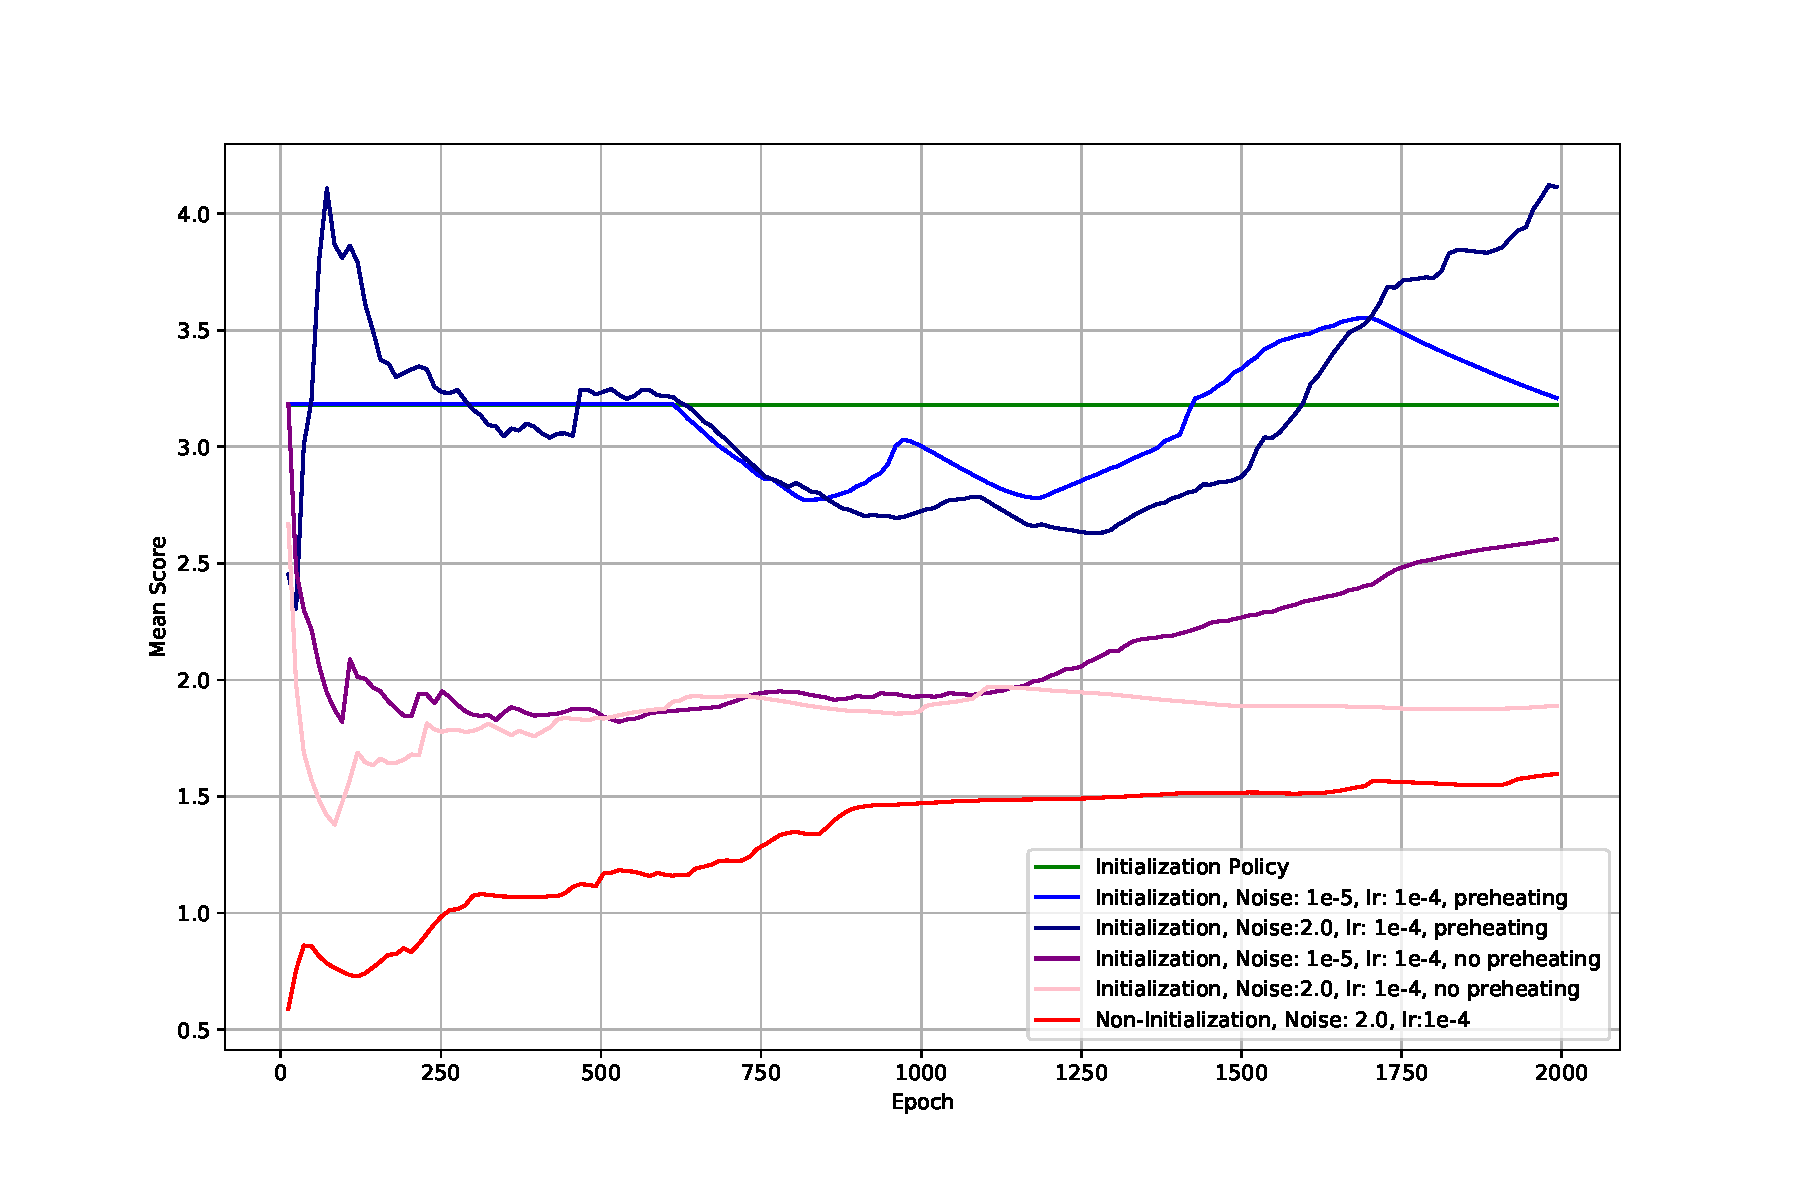
\includegraphics[scale=0.5]{img/ddpg_compare2.pdf}
	\caption{Comparison of initialized DDPG with/without pre-training the critic on \textit{Reacher} task. The green line is the mean reward of initial policy trained with supervised learning.}
	\label{fig:pretrain}
\end{figure}


\subsubsection{PPO}


\subsection{Meta-learning as Initialization for Reinforcement Learning}

\subsubsection{MAML and Reptile}

\subsubsection{Reptile + PPO}







%%%%%%%%%%%%%%%%%
%   Problem 2   %
%%%%%%%%%%%%%%%%%
\pagebreak
\section{Problem 2}

Example of Simplex tableau:
\begin{align}
    \begin{array}{c | cccccc | c}
         BV  & z & x_1 & x_2 & x_3 & x_4 & x_5 & RHS \\ 
         \hline % horizontal line
         z   & 1 & 0 & 0 & -\tfrac{2}{5} & -\tfrac{1}{5} & 0 & -8 \\
         x_2 & 0 & 0 & 1 & -\tfrac{1}{5} & \tfrac{2}{5}  & 0 & 5 \\
         x_5 & 0 & 0 & 0 & -\tfrac{3}{5} & \tfrac{1}{5}  & 1 & 1 \\
         x_1 & 0 & 1 & 0 & \tfrac{3}{5}  & -\tfrac{1}{5} & 0 & 3
    \end{array}
\end{align}


We can define the \LaTeX{} commands \texttt{Tstrut} and \texttt{Bstrut} to get more spacing between rows in the tableau and make it look nicer:
\begin{align}
    \begin{array}{c | cccccc | c}
         BV  & z & x_1 & x_2 & x_3 & x_4 & x_5 & RHS \Tstrut\Bstrut \\ 
         \hline
         z   & 1 & 0 & 0 & -\tfrac{2}{5} & -\tfrac{1}{5} & 0 & -8 \Tstrut\Bstrut \\
         x_2 & 0 & 0 & 1 & -\tfrac{1}{5} & \tfrac{2}{5}  & 0 & 5  \Tstrut\Bstrut \\
         x_5 & 0 & 0 & 0 & -\tfrac{3}{5} & \tfrac{1}{5}  & 1 & 1  \Tstrut\Bstrut \\
         x_1 & 0 & 1 & 0 & \tfrac{3}{5}  & -\tfrac{1}{5} & 0 & 3  \Tstrut\Bstrut
    \end{array}
\end{align}

We can colour text and highlight cells in tableau, or just leave them empty:
\begin{align}
    \begin{array}{c | cccccc | c}
         BV  & z & x_1 & x_2 & x_3 & x_4 & x_5 & RHS \Tstrut\Bstrut \\ 
         \hline
         z   & 1 & & & -\tfrac{2}{5} & -\tfrac{1}{5} & & -8 \Tstrut\Bstrut \\
         x_2 & & & \cellcolor{gray!50}1 & -\tfrac{1}{5} & \tfrac{2}{5} & & 5 \Tstrut\Bstrut \\
         x_5 & & & & -\tfrac{3}{5} & \tfrac{1}{5}  & 1 & 1 \Tstrut\Bstrut \\
         x_1 & & \textcolor{red}{1} & & \tfrac{3}{5}  & -\tfrac{1}{5} & & 3 \Tstrut\Bstrut
    \end{array}
\end{align}

Here is how you make vectors and matrices:
\begin{align}
    \mathbf x = \begin{bmatrix} 1 & 2 & 3 \end{bmatrix} = \begin{bmatrix} 1 \\ 2 \\ 3 \end{bmatrix}^\top \\
    \mathbf A = \begin{bmatrix} 1 & 2 & 3 \\ 4 & 5 & 6 \end{bmatrix}^{-1}
\end{align}

Here is a formulation of a linear program:
\begin{align*}
    \min_{x} \quad & c^\top x \\
    \mathrm{s.t.} \quad 
    & A x \leq b \\
    &-1 \leq x_n \leq 1 \,, \quad n = 1, \dots, N
\end{align*}

There is an ocean of Latex questions and answers online. If you have a question, most likely someone else will have asked the same question before. 

\medskip
 
\bibliographystyle{unsrt}
\bibliography{ref}

\end{document}
